\chapter{Języki i technologie webowe}
\PartialToc
%\startcontents[chapters]
%\printcontents[chapters]{}{1}{\section*{\contentsname}}

\section{Droga pakietu w sieci Internet pomiędzy dwoma
węzłami, tj. lista adresów węzłów odwiedzanych przez pakiet}


Droga takiego pakietu zależy od stanu tablic routingu. Jeżeli stosowany jest routing dynamiczny wtedy pierwsza próba wysłania pakietu się nie powiedzie - router nie zna adresu mac celu i musi go odnaleźć w związku z czym porzuca pakiet, natomiast jeśli w tablicy routingu znajduje się już adres mac węzła docelowego pakiet pójdzie dalej. Całość oczywiście zależy od stopnia skomplikowania sieci (np. ilość routerów po drodze).
\\
\\
Ścieżka pakietu w prostej sieci jest bardzo fajnie i obrazowo opisana tutaj:\\
http://jaredheinrichs.com/tracing-packet-flow-between-a-2-switches-and-a-router.html


\vspace{0.4cm}
\noindent 
%%%%%%%%%%%%%%%%%%%%%%%%
\section{Serwery DNS oferują:}
\vspace{0.4cm}
\noindent
\begin{enumerate}
\item Translację nazwy kanonicznej $\rightarrow$ IP
\item Translację odwrotną (Reverse Lookup): IP $\rightarrow$ nazwa
\end{enumerate}
\vspace{0.4cm}
Najważniejsze typy rekordów DNS oraz ich znaczenie:
\begin{description}

\item[A] adres hosta (ipV4) 
\item[AAAA]  adres hosta (ipV6) 
\item[PTR]  	
	rekord wskaźnika - mapuje adres IPv4 lub IPv6 na nazwę kanoniczną hosta. 		Określenie rekordu PTR dla nazwy hosta (ang. hostname) w domenie in-addr.arpa 	(IPv4), bądź ip6.arpa (IPv6), który odpowiada adresowi IP, pozwala na 			implementację odwrotnej translacji adresów DNS (ang. reverse DNS lookup) 
\item[MX] mapuje nazwę domeny DNS na nazwę serwera poczty oraz jego priorytet 
\item[CNAME]	alias nazwy domeny. Wszystkie wpisy DNS oraz poddomeny są 	poprawne także dla aliasu 
\item[TXT]	rekord ten pozwala dołączyć dowolny tekst do rekordu DNS 
\item[NS] Name Server, serwer nazw dla danej strefy 
\item[SOA]    rekord adresu startowego uwierzytelnienia (ang. start of authority record) ustala serwer DNS dostarczający autorytatywne informacje o domenie internetowej 
\end{description}

Narzędzia do odpytywania DSN: host, dig

%%%%%%%%%%%%%%%%%%%%%%%%
\section{Zaznacz prawdziwe stwierdzenie. Protokół HTTP w  wersji 1.1}

\vspace{0.4cm}
\noindent

Podobnie jak większość protokołów sieciowych, HTTP uzywa modelu klient-serwer: klient HTTP otwiera połączenie i wysyła komunikat żądania do serwera HTTP. Serwer następnie zwraca komunikat odpowiedzi, zwykle zawierający zasób, o który został poproszony.
Portem zarezerwowanym dla HTTP jest 80 port TCP oraz rzadziej używane porty 8008 i 8080.\\

\textsc{\textbf{Struktura protokołu HTTP}}

\begin{enumerate}
\item Żądanie
	\begin{enumerate}
	\item{polecenie}
	\item{nagłówki (0 lub więcej)}
	\item pusta linia
	\item dane
	\end{enumerate}
\item Odpowiedź
	\begin{enumerate}
		\item pojedyncza linia statusu: \textit{protokół kod opis}
		\item{nagłówki (0 lub więcej)}
		\item pusta linia
		\item dane
	\end{enumerate}
\end{enumerate}


\textsc{\textbf{Kody statusu}}

\begin{description}
\item[1xx] powiadomienie
\item[2xx] powodzenie – 200 OK
\item[3xx] przekierowanie do innego URI – 301 Moved Permanently
\item[4xx] błąd po stronie klienta – 404 Not Found
\item[5xx] błąd po stronie serwera – 500 Server Error
\end{description}

\textsc{\textbf{metody http}}
\begin{description}

\item[OPTIONS] — pozwala klientowi ustalić opcje i/lub wymagania związane z danym zasobem, albo możliwości danego serwera, nie implikując działań zasobu i nie inicjując pobierania zasobu.
\item[GET] — pobiera informacje zidentyfikowane przez URI, do którego zostało zgłoszone żądanie. Jeżeli URI zidentyfikuje proces wytwarzający dane, to wytworzone dane zostaną zwrócone jako jednostka.

\item[HEAD] — identyczny z GET, z tym że serwer nie zwraca w odpowiedzi treści komunikatu. Metoda ta uzyskuje informacje dotyczące jednostki nie przesyłając samej treści jednostki i jest wykorzystywana do testowania ważności, dostępności oraz niedawnych modyfikacji łączy hipertekstowych.

\item[POST] — żąda, aby serwery przyjmowały jednostkę załączoną w żądaniu,  POST jest wykorzystywany do przypisywania zasobów, do wysyłania komunikatów, do przedkładania danych formularzy, itp.

\item[PUT] — żąda, aby jednostka załączona w żądaniu została zapamiętana pod URI, do którego zostało zgłoszone żądanie. Jeżeli dany zasób wspomniany w URI już istnieje, to przesyłaną jednostkę uznaje się za wersję zmodyfikowaną. Jeżeli URI nie wskazuje na istniejący zasób, a żądający użytkownik może zdefiniować URI jako nowy zasób, to zasób jest tworzony na serwerze.

\item[DELETE] — żąda, aby serwer usunął zasób zidentyfikowany przez URI.

\item[TRACE] — wywołuje zdalną pętlę zwrotną komunikatu żądania. Ostateczny odbiorca żądania odbija otrzymany komunikat z powrotem do klienta. TRACE pozwala klientowi zobaczyć co jest odbierane na drugim końcu łańcucha żądania. Informacja ta może być wykorzystywana do testowania, lub znajdywania uszkodzeń.

\item[CONNECT] — nazwa metody zarezerwowana do wykorzystywania wraz z proxy, który może dynamicznie przełączyć się na pełnienie funkcji tunelu, przy użyciu, na przykład, tunelowania z wykorzystaniem warstwy zabezpieczeń łączy (SSL). Proxy to program pośredniczący, pełniący zarówno funkcję serwera, jak i klienta, w celu zgłaszania żądań w imieniu innych klientów.
\end{description}

\textsc{\textbf{nagłówki}}\\
Z wykładu:
\begin{description}

\item[Klient:] \hfill \\
	\begin{description}
	\item[From]: – zwykle email
	\item[User-Agent:] – identyfikacja klienta: Nazwa/Wersja Host: – HTTP 1.1
	\end{description}
\item[Serwer:] \hfill \\
	\begin{description}
		\item[Server:] - analogicznie jak User-Agent
		\item[Last-Modified:] – Data i godzina modyfikacji zasobu 
		\item[Connetion:] – rodzaj połączenia (close dla HTTP 1.0)
		\item[Content-Type:] – tym MIME, np. text/html, application/octet-stream
		\item[Content-Length:] – rozmiar w bajtach
	\end{description}
\end{description}
\href{http://www.wikiwand.com/pl/Lista_nag%C5%82%C3%B3wk%C3%B3w_HTTP}{Wincyj nagłówków: wiki} 
\\


\textsc{\textbf{wybrane różnice między wersją HTTP 1.0 i 1.1}}
\begin{enumerate}
\item{\textbf{ w 1.1 może być więcej niż 1 request}\\
Nagłówek Keep-Alive jest rozszerzeniem HTTP/1.0. \\
W HTTP/1.1 ten nagłówek nie jest potrzebny, gdyż połączenia Keep-Alive są domyślne (zachowanie zmienia Connection: close)}
\item{\textbf{w  1.1 w zapytaniu można określić hosta docelowego}\\
GET / HTTP/1.1 \\
Host: kis.agh.edu.pl}
\item{\textbf{nowa wersja wprowadza nagłówki If-Unmodified-Since, If-Match, If-None-Match}}

\end{enumerate}





%%%%%%%%%%%%%%%%%%%%%%%%
\section{Do bezpośredniej komunikacji z serwerem WWW służą następujące narzędzia}

\vspace{0.4cm}
\noindent
 \begin{enumerate}
 \item{nc (netcat)} 
 \item{każdy klient protokołu zdalnego logowania (ssh, telnet) ?}
 \end{enumerate}
 
 
%%%%%%%%%%%%%%%%%%%%%%%%
\section{Wskaż prawdziwe stwierdzenia~o poniższym fragmencie kodu XHTML 1.0 Strict}
\begin{lstlisting}[language=html]
	<p><a  href = http://www.agh.edu.pl><br></p>
\end{lstlisting}

\vspace{0.4cm}
\noindent
\begin{enumerate}
\item Wyrażenie  http://www.agh.edu.pl  powinno zostać ujęte~w cudzysłów.  
\item   Znacznik br powinien byc oznaczony jako jednoczesny znacznik otwierajacy~i zamykający poprzez <br/>
\item Brakuje nazwy hiperłącza (pomiędzy <a></a>).
\item Brakuje znacznika zamykającego dla~a, tuż przed zamknięciem p.
\end{enumerate}


%%% PYTANIE 148


\section{Ile zasobów z dyrektywami CSS może być skojarzonych z pojedynczym dokumentem XHTML 1.0 Strict?}
\answer
{Ile zasobów z dyrektywami CSS może być skojarzonych z pojedynczym dokumentem XHTML 1.0 Strict?}
{Zero}
{F}
{Nie ma ograniczenia dołączanych plików styli.}
{Nie ma czego wyjaśniać}

%%% PYTANIE 149
\section{Zaznacz prawdziwe stwierdzenia dotyczące poniższego kodu CSS 2.1.}
\begin{lstlisting}[language=html]
.nav > div {
	color: white;
	background: #119500;
	float: right;
	width: 120px;
	padding: 1px;
	font-size: small;
	border: solid red 1px;
}
\end{lstlisting}

\noindent
{\textbf{Przykładowa odpowiedź:}}
Kolor tła ustalony jest jako wartości składowych RGB, odpowiednio (dziesiętnie) 11, 95, 0.
\textbf{FAŁSZ}

\vspace{0.4cm}
\noindent
\textbf{Odpowiedź:}
Brak jednoznacznej odpowiedzi.

\vspace{0.4cm}
\noindent
\textbf{Wyjaśnienie:}

Powyższa definicja styli dotyczy elementu div, będącego bezpośrednim potomkiem elementu z klasą nav (znaczenie selektora \textbf{>}).
Na przykład:
\begin{lstlisting}[language=html]
<div class="nav">
	<div id="stylowanyDiv"></div>
</div>
\end{lstlisting}

Tu stylowanie nie będzie miało miejsca:

\begin{lstlisting}[language=html]
<div class="nav">
	<span>
		<div id="nieBedeStylowany"></div>
	</span>
</div>
\end{lstlisting}


\begin{itemize}
\item
\textbf{color} - kolor tekstu wewnątrz elementu; w tym przypadku tekst będzie BIAŁY.
\item
\textbf{background} - tło elementu; tutaj ustawiony kolor tła jako wartość HEX koloru. Chcąć ustawiać kolor jako dziesiętne wartości RGB używamy formy rgb(R, G, B)
\item
\textbf{float} - w najprostszej formie określa czy i jak element będzie 'opływany' przez tekst; tutaj, div będzie znajdował się po prawej stronie, a tekst z lewej.
\item
\textbf{width} - szerokość elementu blokowego; tutaj, 120 px
\item
\textbf{padding} - jest odstępem między zawartością elementu a jego wewnętrzną krawędzią; tutaj, 1px dla wartości górnej, prawej, dolnej i lewej jednakowo.
\item
\textbf{font-size} - rozmiar tekstu; tutaj, mniejsza niż domyślna. Dokładny rozmiar jest zależny od przeglądarki.
\item
\textbf{border} - obramowanie elementu; solid - linia ciągła, red - czerwony kolor obranowania, 1px - grubość obramowania;
\end{itemize}
\begin{center}
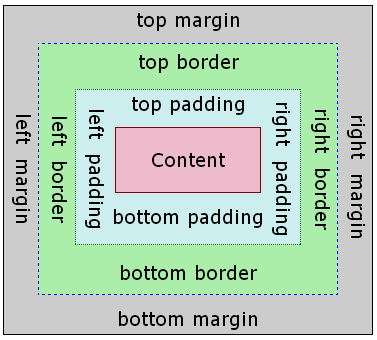
\includegraphics[width=6cm]{09/boxmodel}
\captionof{figure}{Model pudełkowy elementów strony}
\end{center}

\textbf{!UWAGA!: }120px jest poprawne; 120 px już nie!


%%% PYTANIE 150
\section{Wskaż prawdziwe stwierdzenia odnośnie poniższego fragmentu kodu PHP.}
\begin{lstlisting}[language=php]
$fp = fopen("plik_do_blokowania", "r+");
if(flock($fp, LOCK_EX)) {
	processing();
	flock($fp, LOCK_UN);
} else {
	problem();
}
fclose($fp);
\end{lstlisting}

\noindent
{\textbf{Przykładowa odpowiedź:}}
Funkcja \textit{processing()} jest wywoływana w sekcji krytycznej.
\textbf{PRAWDA}

\vspace{0.4cm}
\noindent
\textbf{Odpowiedź:}
Brak jednoznacznej odpowiedzi.

\vspace{0.4cm}
\noindent
\textbf{Wyjaśnienie:}

\begin{enumerate}
\item 
Funkcja \textit{fopen} przyjmuje jako pierwszy argument ścieżkę do pliku, który ma zostać otwarty, a jako drugi - tryb otwarcia, jak niżej:
\begin{itemize}
\item
\textbf{r} - otwiera plik do odczytu
\item
\textbf{r+} - otwiera plik do odczytu i zapisu
\item
\textbf{w} - kasuje zawartość pliku i otwiera go do zapisu
\item
\textbf{w+} - kasuje zawartość pliku i otwiera go do zapisu i odczytu
\item
\textbf{a} - otwiera plik do dopisywania
\item
\textbf{a+} - otwiera plik do dopisywania i odczytu
\end{itemize}
Zwraca wartość liczbową identyfikującą otwarty plik.
\item
Funkcja \textit{fclose} służy do zamknięcia pliku otwartego wcześniej przez fopen. Jako argument przyjmuje liczbowy identyfikator pliku, który ma zostać zamknięty.
\item
Funkcja \textit{flock} służy do zarządzania blokowaniem dostępu do pliku jako zabezpieczenie podczas współdzielenia pliku. Zapobiega to równoczesnej modyfikacji pliku przez kilka osób/wątków.
\begin{itemize}
\item
\textbf{LOCK\_SH} - dostęp do odczytu; inne wątki mogą czytać plik, ale nie mogą zablokować go do zapisu. Zapobiega to odczytowi niepełnych danych przez inne wątki i wprowadzeniu zmian w pliku czytanym przez inne wątki.
\item
\textbf{LOCK\_EX} - dostęp do zapisu; wątek blokując plik w ten sposób ma go 'na wyłączność'. Inne wątki nie mogą go odczytać, a tym bardziej zapisać. Zapobiega wprowadzaniu zmian przez kilka wątków jednocześnie oraz odczytania niepełnych (przed edycją) danych.
\item
\textbf{LOCK\_UN} - zwolnienie blokady 
\item
\textbf{LOCK\_NB} - Gdy ustawiona, proces który natknął się na blokadę nie będzie czekał na swoją kolej. Używa się tej opcji w połączeniu, z którąś opcją blokady np. \textit{flock(\$fp, LOCK\_EX | LOCK\_NB)}. Użyta w naszym przypadku pozwoliła by na przejście bo bloku \textit{else} gdy plik jest już zablokowany, zamiast czekać na zwolnienie.\textbf{LOCK\_UN}
\end{itemize}
\textit{flock} zwraca true w przypadku sukcesu i false w przeciwnym razie.
Gdy \textit{flock} nie może uzyskać do zasobu, oczekuje na zwolnienie blokady przez inny wątek!

Funkcja \textit{flock} może przyjmować także opcjonalnie trzeci parametr. Jego wartość jest ustawiana jako 1, gdy proces zostanie zablokowany (nie uzyska dostępu do pliku). Głównie służy do sprawdzenia czy coś złego się nie wydarzyło - gdy funkcja zwraca \textbf{false}, a trzeci parametr ma wartość 0, oznacza to że wystąpił jakiś błąd, ponieważ \textit{flock} nie mógł uzyskać blokady, a jednak proces nie został wstrzymany przez już istniejącą blokadę na pliku.
\end{enumerate}


\textbf{Analiza kodu:}
\begin{enumerate}
\item
Otwieramy plik "plik\_do\_blokowania" w celu odczytu i zapisu. Identyfikator przypisujemy do zmiennej \$fp.
\item
Następnie próbujemy uzyskać dostęp do pliku w trybie exclusive.
Jeżeli plik nie został wcześniej zablokowany ani do odczytu, ani zapisu przez inny wątek - funkcja \textit{flock} zwraca \textbf{true} i blokuje plik.
\item
Wówczas wchodzimy w sekcję krytyczną gdzie aktywowana jest funkcja \textit{processing()}.
\item
Po jej wykonaniu blokada pliku jest zwalniana poprzez \textit{flock(\$fp, LOCK\_UN)}.
\item
Jeżeli plik jest odczytywany lub zapisywany przez inny wątek (został wcześniej zablokowany) funkcja \textit{flock} zwraca \textbf{false}.
Wówczas \textit{flock} oczekuje na zwolnienie blokady przez inny wątek; czeka na swoją kolej.
\item
Po wykonaniu powyższych czynności plik zostaje zamknięty.
\end{enumerate}

\textbf{!Uwaga!: }Tak naprawdę, w tym przykładzie nie wejdziemy do bloku 'else'!

%%%% Pytanie 151
\section{Zawartość poniższego formularza przesłano do skryptu PHP. Zaznacz prawdziwe stwierdzenia.}
\begin{lstlisting}[language=html]
<form action="skrypt.php" method="post" enctype="multipart/form-data">
	<p>
		<input type="file" name="plik"/>
		<input type="text" name="comment" />
		<input type="submit" value="wyslij" />
	</p>
</form>
\end{lstlisting}

\noindent
{\textbf{Przykładowa odpowiedź:}}
W zmiennej \textit{\$\_POST['comment']} będzie dostępna zawartość pola tekstowego.
\textbf{PRAWDA}

\vspace{0.4cm}
\noindent
\textbf{Odpowiedź:}
Brak jednoznacznej odpowiedzi.

\vspace{0.4cm}
\noindent
\textbf{Wyjaśnienie:}
Formularz php składający się z trzech elementów:
\begin{enumerate}
\item
Kontrolka do uploadu pliku. Klikając klawisz pojawi się okno eksploratora i można wybrać plik z dysku. Zmienna z nim związana nazwana została 'plik'.
\item
Pole tekstowe, umożliwiające wpisanie tekstu przez użytkownika. Pierwotnie pole tekstowe jest puste. Zmienna z nim związana nazwana została 'comment'.
\item
Klawisz zatwierdzający formularz. Po jego wciśnięciu dane z formularza zostają wysłane do skryptu 'skrypt.php' metodą POST.
\end{enumerate}

Parametr \textbf{enctype} określa w jaki sposób dane z formularza zostaną przekształcone. Może być użyty TYLKO w połączeniu z \textbf{method="POST"}.
	Możliwe wartości:
\begin{itemize}
\item
\textbf{application/x-www-form-urlencoded} - DOMYŚLNE; Wszystkie dane są przekształcane. Spacje zmieniane na +, znaki specjalne zmieniane na wartości ASCII HEX.
\item
\textbf{multipart/form-data} - żadne znaki nie są przekształcane; wymagany w przypadku użycia w formularzu kontrolki typu \textbf{'file'}
\item
\textbf{text/plain}- spacje są przekształcane na znak +, znaki specjalne nie są przekształcane
\end{itemize}

Po stronie skryptu php dostępne są wartości z tablicy asocjacyjnej \textit{\$\_POST} (pola z formularza z metodą \textbf{POST}; przy użyciu metody \textbf{GET} wartości dostępne są spod \textit{\$\_GET}) oraz \textit{\$\_FILES} (dane z kontrolki typu \textbf{file}).

\begin{itemize}
\item
\$\_POST: Array ([comment] => <tresc\_komentarza\_wpisana\_w\_polu>)
\item
\$\_FILES: Array ([plik] => Array ([name] => <nazwa\_pliku> [type] => image/png [tmp\_name] => <sciezka\_do\_pliku\_w\_tempie> [error] => 0 [size] => 38676))
\end{itemize}
Do elementów dostać się można na przykład: \textit{\$\_POST['comment']}, \textit{\$\_FILES['plik']['name']}.

Elementy formularza zgrupowane są wewnątrz znacznika akapitu (<p>).

%%%%%%%%%%%%%%%%%%%%%%%%
\section{Co jest efektem działania poniższego programu~w języku PHP.}
\textbf{Co jest efektem działania poniższego programu~w języku PHP.}
\begin{lstlisting}[language=php]
	<?php
	$wiek = array('ala'  => 12, 'ela' => 22, 'franek' => 54);
	foreach ($wiek as $k =>$w)
		echo $k.' '.$w."\n";
	?>
\end{lstlisting}
\vspace{0.4cm}
\noindent
Tablice~w PHP działają jak mapy, mają pary kluczy wraz~z wartościami.~W związku~z tym zostanie wypisany następujący ciąg:

ala  12

ela  22

franek  54
\vspace{0.4cm}

%%%%%%%%%%%%%%%%%%%%%%%%
\section{Jak długi będzie czas wykonania poniższego programu napisanego w języku PHP?}
\textbf{Zakłada się, że program uruchamiany jest jako aplikacja WWW tj. dostępny jest pod określonym adresem URI, a interpreter PHP uruchamiany jest przez serwer WWW.}

\begin{lstlisting}[language=php]
1 <? php
2 echo 'start';
3 sleep(6);
4 ?>

\end{lstlisting}

Wywołanie \textbf{sleep(6)} powoduje "uśpienie" programu na 6 sekund. Do tego czasu należy doliczyć także czas wykonania instrukcji \textbf{echo 'start'}, więc ogólny czas wykonania programu będzie większy niż 6 sekund. Sprawdzone za pomocą funkcji \textbf{microtime()}.

\vspace{0.4cm}
\noindent

%%%%%%%%%%%%%%%%%%%%%%%%
\section{Która~z poniższych metod~w języku JavaScript zwraca element~o unikalnym identyfikatorze form?}

\begin{lstlisting}[language=html]
	document.getElementById('form').
\end{lstlisting}


%%%%%%%%%%%%%%%%%%%%%%%%
\section{Zaznacz prawdziwe stwierdzenia dotyczące poniższego kodu~w języku JavaScript}

\begin{lstlisting}[language=html]
		car = new Array();
		car[0] = new Object();
		car[0].make = 'Fiat';
		car[0].vin = '123';
		car[1] = new Object();
		car[1].make = 'Ford';
		car[1].vin = '456';
		
		for(idx in car){
			for(prop in car [idx]){
				document.write(car[idx][prop]);
			}
		}
\end{lstlisting}

\vspace{0.4cm}
\noindent
Pierwsza pętla operuje po obiektach,~a druga po ich wartościach.~W związku~z tym zostanie wypisane: Fiat123Ford456 (~w miejscu,~w którym został wstawiony kod).

%%%%%%%%%%%%%%%%%%%%%%%%
\section{Zaznacz prawdziwe stwierdzenia dotyczące poniższego kodu w języku JavaScript.}



\begin{lstlisting}
function updateAjax() {
    xmlhttp = new XMLHttpRequest();
    xmlhttp.onreadystatechange = function() {
        if (xmlhttp.readyState == 4 && xmlhttp.status == 200) {
            document.getElementById("stime").innerHTML = xmlhttp.responseText;
        }
    }
    xmlhttp.open("GET", "date.php", true);
    xmlhttp.send();
    window.setTimeout("updateAjax()", 1000);
}
window.setTimeout("updateTime(); updateAjax();", 5000);
\end{lstlisting}

\begin{itemize}
\item{Event \textbf{XMLHttpRequest.onreadystatechange} jest triggerowany za każdym razem, gdy
\textbf{XMLHttpRequest.readyState} się zmienia}

\item{\textbf{XMLHttpRequest.readyState == 4} oznacza, że wysłany przez nas request został zakończony.}

\item{\textbf{XMLHttpRequest.status == 200 } (HTTP status 200) oznacza, że nasz request został przetworzony poprawnie}

\item{\textbf{XMLHttpRequest.responseText} jest odpowiedzią serwera na nasz request. W przypadku powyższego kodu elementowi \textbf{na naszej stronie} o id == 'stime' zostanie przypisana odpowiedź serwera.} 

\item{Funkcja \textbf{XMLHttpRequest.open(method,url,async)} określa typ requestu jaki zostanie wysłany. }

\item{\textbf{window.setTimeout(function, milliseconds)} powoduje pojedyncze uruchomienie funkcji (jak widać w powyższym kodzie może ich być kilka) określonej przez parametr \textbf{function} po odczekaniu czasu określonego przez parametr \textbf{miliseconds}.}

\end{itemize}
Komunikacja AJAX rozpocznie się po 5 sekundach od zinterpretowania kodu. Następnie funkcja \textbf{updateAjax()} będzie wywoływana co jedną sekundę (sama ustawia sobie timeout).


\vspace{0.4cm}
\noindent

%%%%%%%%%%%%%%%%%%%%%%%%%%%
\section{Dany jest dokument XML oraz odpowiednie DTD. Zaznacz prawdziwe stwierdzenia.}


\textbf{DTD} -  rodzaj dokumentu definiujący formalną strukturę dokumentów XML, HTML, XHTML lub innych
 pochodzących z rodziny SGML lub XML. Definicje DTD mogą być zawarte w pliku dokumentu, którego strukturę definiują, przeważnie jednak zapisane są w osobnym pliku tekstowym, co pozwala na zastosowanie tego samego DTD dla wielu dokumentów.\\

\textbf{XMLSchema} - opracowany przez W3C standard służący do definiowania struktury dokumentu XML. XML Schema stanowi alternatywę dla DTD, przy czym posiada znacznie większe możliwości. XML Schema jest strukturą XML, w odróżnieniu od DTD nie będącego częścią standardu XML. Dokumenty zawierające definicje XML Schema zapisuje się zwykle w plikach z rozszerzeniem .xsd (od XML Schema Definition).
\\
\\
\textbf{Funkcjonalność DTD może zostać zastąpiona przez XMLSchema. Należy jednak pamiętać, że składnia XMLSchema sama w sobie jest zazwyczaj definiowana przez DTD.}\\
\\
Dokładniejszy opis różnic pomiędzy DTD a XMLSchema oraz ich składnię można podejrzeć tutaj:\\
http://www.sitepoint.com/xml-dtds-xml-schema/